%%%%%%%%%%%%%%%%%%%%%%%%%%%%%%%%%%%%%%%%%
% Beamer Presentation
% LaTeX Template
% Version 1.0 (10/11/12)
%
% This template has been downloaded from:
% http://www.LaTeXTemplates.com
%
% License:
% CC BY-NC-SA 3.0 (http://creativecommons.org/licenses/by-nc-sa/3.0/)
%
%%%%%%%%%%%%%%%%%%%%%%%%%%%%%%%%%%%%%%%%%

%----------------------------------------------------------------------------------------
%   PACKAGES AND THEMES
%----------------------------------------------------------------------------------------

\documentclass{beamer}

\mode<presentation> {

% The Beamer class comes with a number of default slide themes
% which change the colors and layouts of slides. Below this is a list
% of all the themes, uncomment each in turn to see what they look like.

%\usetheme{default}
%\usetheme{AnnArbor}
%\usetheme{Antibes}
%\usetheme{Bergen}
%\usetheme{Berkeley}
%\usetheme{Berlin}
%\usetheme{Boadilla}
%\usetheme{CambridgeUS}
%\usetheme{Copenhagen}
%\usetheme{Darmstadt}
%\usetheme{Dresden}
%\usetheme{Frankfurt}
%\usetheme{Goettingen}
%\usetheme{Hannover}
%\usetheme{Ilmenau}
%\usetheme{JuanLesPins}
%\usetheme{Luebeck}
\usetheme{Madrid}
%\usetheme{Malmoe}
%\usetheme{Marburg}
%\usetheme{Montpellier}
%\usetheme{PaloAlto}
%\usetheme{Pittsburgh}
%\usetheme{Rochester}
%\usetheme{Singapore}
%\usetheme{Szeged}
%\usetheme{Warsaw}

% As well as themes, the Beamer class has a number of color themes
% for any slide theme. Uncomment each of these in turn to see how it
% changes the colors of your current slide theme.

%\usecolortheme{albatross}
%\usecolortheme{beaver}
%\usecolortheme{beetle}
%\usecolortheme{crane}
%\usecolortheme{dolphin}
%\usecolortheme{dove}
%\usecolortheme{fly}
%\usecolortheme{lily}
%\usecolortheme{orchid}
%\usecolortheme{rose}
%\usecolortheme{seagull}
%\usecolortheme{seahorse}
%\usecolortheme{whale}
%\usecolortheme{wolverine}

%\setbeamertemplate{footline} % To remove the footer line in all slides uncomment this line
%\setbeamertemplate{footline}[page number] % To replace the footer line in all slides with a simple slide count uncomment this line

%\setbeamertemplate{navigation symbols}{} % To remove the navigation symbols from the bottom of all slides uncomment this line
}

\usepackage{graphicx} % Allows including images
\usepackage[utf8]{inputenc}
\usepackage[russian]{babel}
\usepackage{booktabs} % Allows the use of \toprule, \midrule and \bottomrule in tables

%----------------------------------------------------------------------------------------
%   TITLE PAGE
%----------------------------------------------------------------------------------------

\title[Суммы покупок]{Отчет по заданию \textnumero1 курса АМА: \\ Суммы покупок} % The short title appears at the bottom of every slide, the full title is only on the title page

\author{Оспанов Аят} % Your name
\institute[] % Your institution as it will appear on the bottom of every slide, may be shorthand to save space
{
517 группа \\ % Your institution for the title page
}
\date{} % Date, can be changed to a custom date

\begin{document}

\begin{frame}
\titlepage % Print the title page as the first slide
\center{Москва, 2016}
\end{frame}

% \begin{frame}
% \frametitle{Overview} % Table of contents slide, comment this block out to remove it
% \tableofcontents % Throughout your presentation, if you choose to use \section{} and \subsection{} commands, these will automatically be printed on this slide as an overview of your presentation
% \end{frame}

%----------------------------------------------------------------------------------------
%   PRESENTATION SLIDES
%----------------------------------------------------------------------------------------

%------------------------------------------------
\section{First Section} % Sections can be created in order to organize your presentation into discrete blocks, all sections and subsections are automatically printed in the table of contents as an overview of the talk
%------------------------------------------------

% \subsection{Subsection Example} % A subsection can be created just before a set of slides with a common theme to further break down your presentation into chunks

\begin{frame}
\frametitle{Рассмотренные алгоритмы}
Весовые схемы:
\begin{itemize}
\item Линейные с параметром степени: \\ $w_i^0 = \big(\frac{d - i + 1}{d}\big) ^ \delta, i \in \{1, ..., d\}, \delta \in [0; +\infty)$
\item Обратно-степенные: \\ $w_i^1 = \frac{1}{i ^ \gamma}, i \in \{1, ..., d\}, \gamma \in [0; +\infty)$
\end{itemize}

Обучение проходило по всем данным, кроме последней известной покупки. Контроль на последнем известном дне покупки.
\end{frame}

%------------------------------------------------

\begin{frame}
\frametitle{Обработка данных}
Создавался календарь для каждого пользователя и удалялись недели, на которых не было покупок. Календарь - матрица $N x 7$. Создавался календарь для дальнейшего упрощения подсчетов.
\end{frame}

%------------------------------------------------

\begin{frame}
\frametitle{Первая попытка}
Пусть D - день недели, на который нужно предсказать покупку пользователя, $s_i, i \in \{1, ..., d\}$ - покупки пользователя в D-й день i-й недели, $S_i, i \in \{1, ..., n\}$ - все покупки пользователя.

Тогда покупка пользователя на D-й день определяется по следующей схеме:
$$s = \alpha * \frac{\sum_{i=1}^{d} s_i}{d} + (1 - \alpha) * \frac{\sum_{i=1}^{n} S_i}{n}$$

Такая схема при $\alpha = 0.8$ дала MAE = 277.86249 на Public
\end{frame}

%------------------------------------------------

\begin{frame}
\frametitle{Вторая попытка}
На этот раз применялись весовые схемы и их комбинации

Покупка пользователя на D-й день определяется по следующей схеме:
$$s = \alpha * \sum_{i=1}^{d} w_i^0 * s_i + \beta * \sum_{i=1}^{d} w_i^1 * s_i + (1 - \alpha - \beta) * \frac{\sum_{i=1}^{n} S_i}{n}$$

\end{frame}

%------------------------------------------------

\begin{frame}
\frametitle{Настройка параметров}
Настройка параметров велась минимизируя MAE на последнем известном дне. Побдор проходил в два этапа:
\begin{itemize}
\item Подбор $\delta, \gamma$ при фиксированных $\alpha, \beta$
\item Подбор $\alpha, \beta$ при фиксированных $\delta, \gamma$
\end{itemize}

\end{frame}

%------------------------------------------------

\begin{frame}
\frametitle{Подбор $\delta, \gamma$}

\begin{figure}
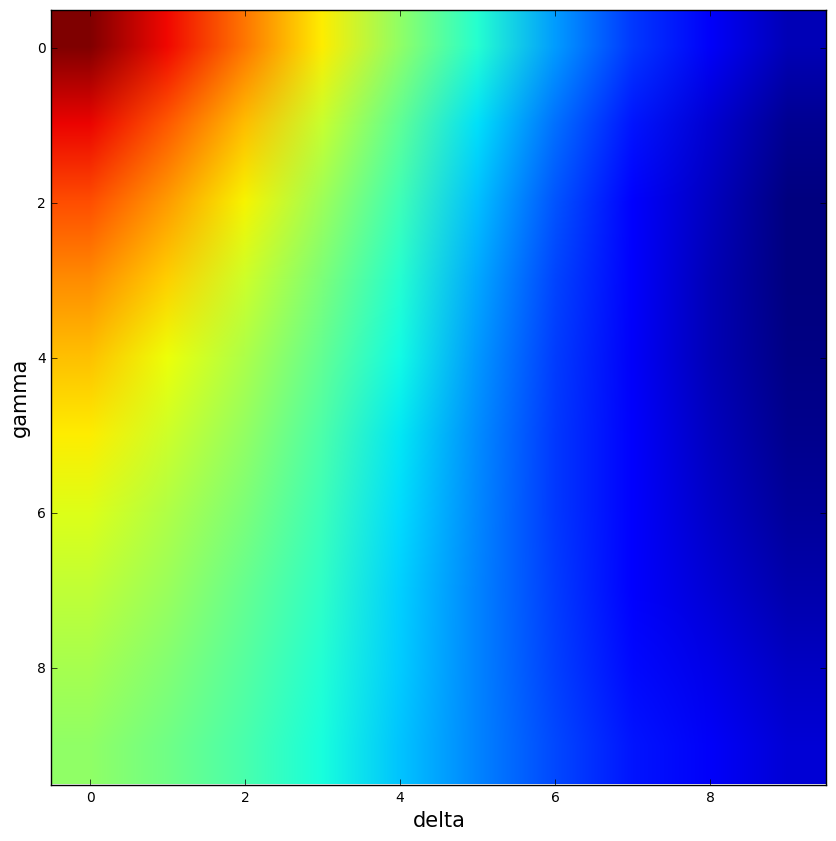
\includegraphics[height=0.5\linewidth]{pics/gamma-delta.png}
\end{figure}

\end{frame}

%------------------------------------------------

\begin{frame}
\frametitle{Подбор $\alpha, \beta$}

\begin{figure}
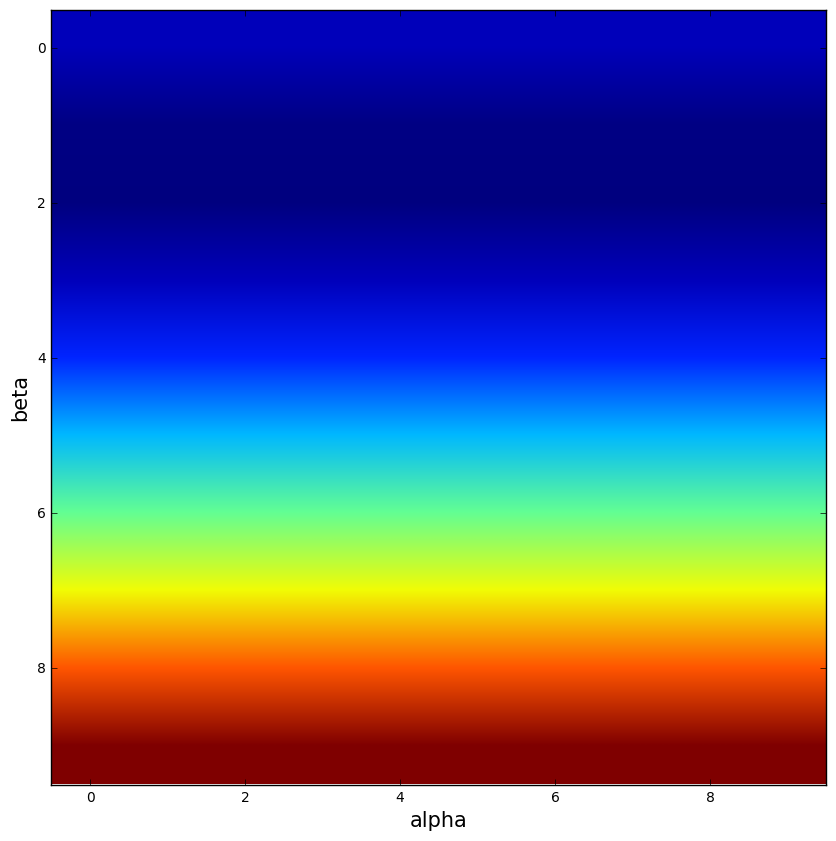
\includegraphics[width=0.5\linewidth]{pics/beta-alpha.png}
\end{figure}

\end{frame}

%------------------------------------------------

\begin{frame}
\frametitle{Результаты подбора параметров}

В итоге оптимизаций получились следующие параметры:
$$\delta = 0.375, \gamma = 3.33, \alpha = 0.42, \beta = 0.33$$
$$MAE = 244.41844$$

Но это привело к тому, что мы переобучились. Public score при этих параметрах дал
$$MAE = 281.68734$$

В связи с этим, встала проблема побдора параметров. Решилось это эмпирическим путем, что привело к
$$\delta = 0.5, \gamma = 0.72, \alpha = 0.22, \beta = 0.44$$
$$MAE = 275.88369$$

\end{frame}

%------------------------------------------------

\begin{frame}
\frametitle{Итог}

Были опробованы весовые схемы предсказания суммы следующей покупки. Т.к. второй метод является более параметризируемым, удалось достигнуть неплохого результата. Но второй метод не идеален, т.к. имеет 4 гиперпараметра, что может привести к переобучению. Также выяснилось, что нужен талант и везение, чтобы настроить гиперпараметры =)

\end{frame}

%------------------------------------------------

\begin{frame}
\LARGE{\centerline{Спасибо за внимание!}}
\end{frame}

%----------------------------------------------------------------------------------------

\end{document}